\documentclass{scrartcl}

\usepackage{hyperref}
\usepackage{graphicx}
\graphicspath{./}

\title{Distinguishing Key Points Useful for Hotel Recognition}
\subtitle{Neural Networks Course Project Redirection and Progress Update}
\date{December 2021}
\author{
  Oliver Broadrick\\
  \texttt{obroadrick@gwu.edu}
  \and
  Marshall Thompson
}

\begin{document}

\maketitle

\section{Outline}

Since the course of our project has shift directions substantially since we began, we are creating this document to serve as an update on both 
\begin{enumerate}
\item
The new direction and associated goals of the project,
\item
The progress that we have made on these new goals.
\end{enumerate}

\section{Brief Background: Hotel Recognition}
We are moving in a new direction, although the content is largely the same. As noted in \href{./initial_proposal.pdf}{our previous neural networks course project proposal}, we are working on a project outside of this class involving fighting sex trafficking. In sex trafficking cases, images are sometimes available of victims in hotel rooms. If, given such an image (or images), it can be determined the hotel chain, or even specific location, in which the image is taken, then this can be used to bust cases, catch perpetrators, and prosecute. Successful completion of this hotel recognition task can save lives.

The search utility Traffickcam already exists to help solve this problem, but Marshall and I (with two other GW peers) are working on developing a new search algorithm that makes use of key points in the image. While the current Traffickcam algorithm uses a single vector description of each whole image, our approach allows descriptors of many small patches in images that could be used as identifiers for the hotel. Since large portions of query images are masked due to sensitive content, using keypoints may result in more accurate and reliable search results.


\section{Distinguishing Key Points as a Neural Networks Problem}
The main issue with directly searching over all of the key points for all of the images in the database comes from scale. It is simply too computationally expensive to, at query time, do a brute for search over all the points we have. With roughly 10 million images, each with roughly 1 thousand points, we have a total of about 10 billion points in our database. Through testing with images from known hotels, we have found that the very closest matching points are the ones that allow us to distinguish the hotel from which an image comes. This realization, in addition to intuition about the specifics of hotel rooms, is what leads us to the conjecture that some key points are generally good for hotel recognition, while some key points are generally bad for hotel recognition.

\begin{figure}
\begin{center}
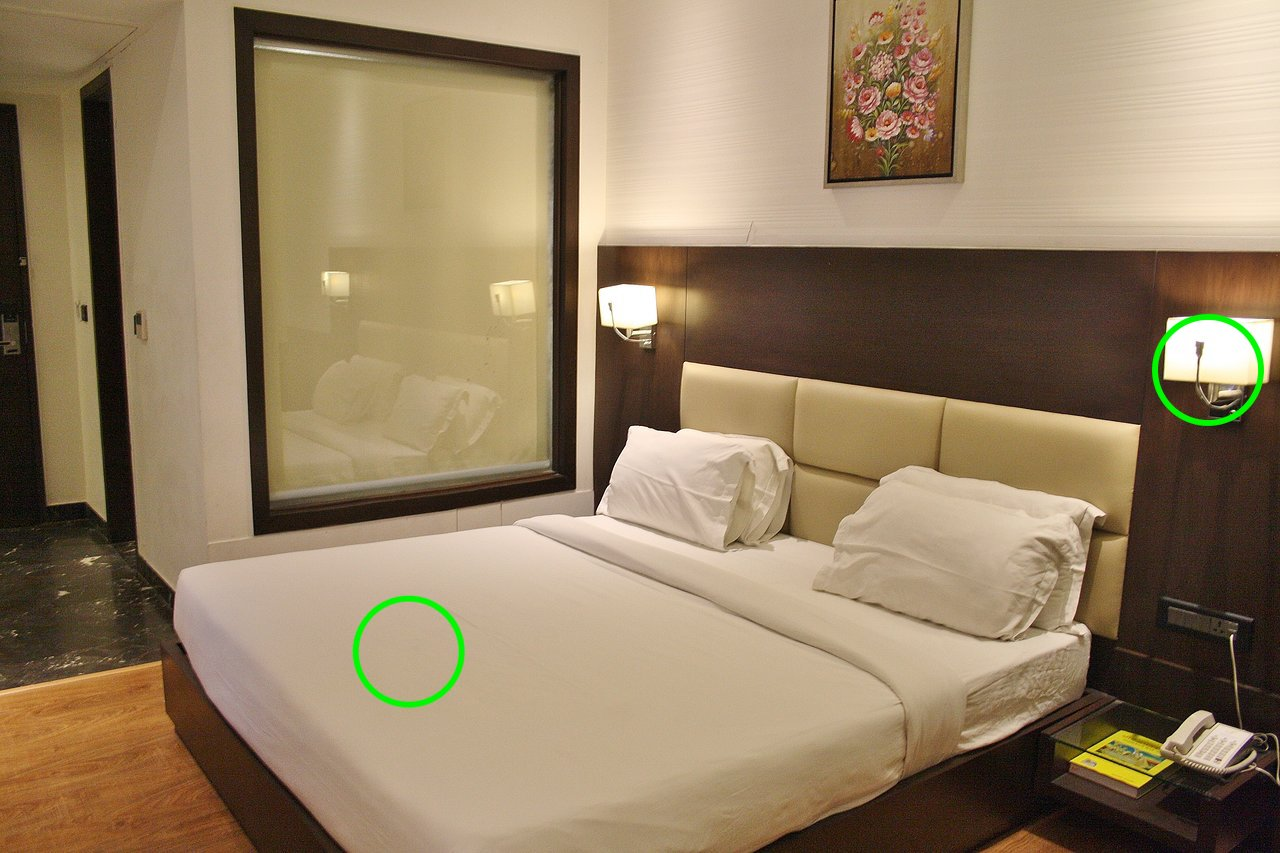
\includegraphics[scale=.3]{goodbadpoint_hotel}
\end{center}
\caption{An image from a hotel room, with two circles showing possible key points in the image.}
\label{img}
\end{figure}

For the example query image in \ref{img}, the point on the right is on a lamp, one which may be unique to the hotel chain or specific hotel in which the image was taken. On the other hand, the point on the left is on the plain white bed sheets, a color and texture which is likely to appear in many hotels from many locations and chains. Thus, we would like to describe the point on the right as a good point and point on the left as a bad point, within the context of hotel recognition. 

The key points we are using, R2D2 points, have 128-dimension vector descriptors. To measure the similarity of two points we use cosine similarity. Consider the more abstract, 2-dimensional representation of our problem below. In this abstract example, again point P1 is a point which we would consider good because the nearest point from the same hotel is near but the nearest point from a different hotel is far. On the other hand, point P2 is bad because, while it is just as near to a point from the same hotel at P1, the nearest point in a different hotel is also quite near.

\begin{figure}
\begin{center}
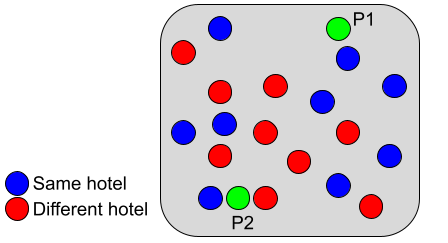
\includegraphics[scale=.7]{points_diagram}
\end{center}
\caption{A diagram showing points in a plane. The points give a toy example of our search space, with two points (P1 and P2) from a query image, and blue points from the same hotel as the query image, and red points from a different hotel.}
\label{dia}
\end{figure}

Here we are led to the way which we will construct labels for our training data. We will compute, for each point in our training set, the nearest point among all points in the same hotel and the nearest point among all points in different hotels. The ratio of these two distances will serve as the metric by which we judge good and bad points. This metric will allow us to choose the best cutoff for distinguishing between the good and bad points based on the distribution over all the points for which we compute the ratio. After choosing the cutoff, we will have a training set of points with their labels. 

One additional item worth noting from Figure \ref{dia} is that we do not expect points from a hotel to be neatly clustered together. That is to say, we do not expect that all points in the same hotel are similar. Rather, we hope that for each hotel, there are certain points which are more unique than others and thus serve better for finding matches than others do. This is to say, that the typical concept of clusters and finding the cluster to which a query vector belongs does not easily or neatly apply to this problem. We will begin testing with a simple binary classification model in Keras, and we will fine tune the particular parameters of the model through testing and evaluating on our abundant data (9 billion points).


\section{Progress}

We have already obtained our dataset, the same one as presented in Hotels-50K. We have also already computed, on all 9 million images in the dataset, all of the R2D2 points that have a confidence score of at least .95. We have written scripts for interfacing with this data, which is currently stored on a GW research server in Pickl files. We have also written a script which is currently running to do the brute force computation of all cosine similarities for a small subset of the total images. That script is then computing the ratio of the distance from the nearest point in the same hotel to the nearest point in a different hotel, as described in the previous section. Finally, the script is storing these ratios for easy plotting afterwards. 

We will, after the script has finished running, choose a cutoff above which we label points good and below which we label them bad, perhaps average, median, or some higher quantile. These few cutoffs can then be used for labeling, training, and testing of our model. The basic outline of our model has already been written in Python using Keras. We intend to report on the testing of various parameters that we tweak (including how we choose the cutoff point). We, of course, hope that our predictions hold true, and we are ultimately able to demonstrate our working model on some testing data from the database.

\begin{thebibliography}{9}
\bibitem{hotels-50k}
\href{https://www2.seas.gwu.edu/~pless/papers/Hotels50k.pdf}{
Pless et al. (2021) Hotels-50k: A Global Hotel Recognition Dataset
}

\bibitem{r2d2}
\href{https://europe.naverlabs.com/research/publications/r2d2-reliable-and-repeatable-detectors-and-descriptors-for-joint-sparse-local-keypoint-detection-and-feature-extraction/}{
Revaud et al. (2019) R2D2: Repeatable and reliable detector and descriptor
}

\end{thebibliography}


\end{document}